\section{Photovoltaic Implant}

%% TODO: rivedere questa parte
%% tutto preso da
% https://extension.arizona.edu/sites/extension.arizona.edu/files/pubs/az1742-2018.pdf
Solar photovoltaic (PV) energy systems are made up of
different components. Each component has a specific role.
The type of component in the system depends on the type
of system and the purpose. For example, a simple PV-direct
system is composed of a solar module or array (two or more
modules wired together) and the load (energy-using device)
it powers. A solar energy system produces
direct current (DC). This is electricity which travels in one
direction. The loads in a simple PV system also operate
on direct current (DC). A stand-alone system with energy
storage (a battery) will have more components than a PV-
direct system.

\subsection{Solar Module}
The majority of solar modules available on the market and
used for residential and commercial solar systems are silicon-
crystalline. These modules consist of multiple strings of solar
cells, wired in series (positive to negative), and are mounted
in an aluminum frame. The size or area of
the cell determines the amount of amperage. The larger the
cell, the higher the amperage.

\begin{figure}[H]
    \centering
    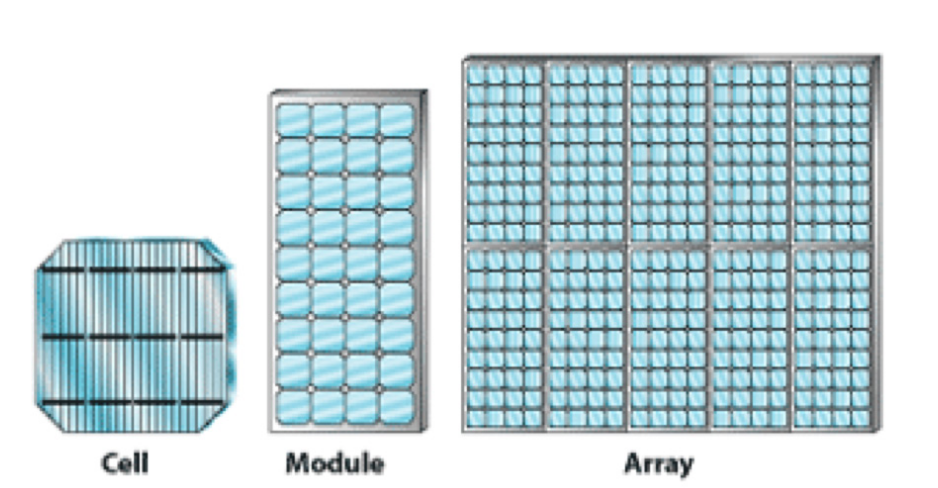
\includegraphics[width=10cm, keepaspectratio]{chapters/1_introduction/imgs/solarmodule.png}
    \caption{The solar cell is the basic component. Cells wired together
and mounted in a frame compose a solar module. Several modules
wired together form an array.}
    \label{fig:solmodule}
\end{figure}

\subsection{Solar Array}
The solar array is made up of multiple PV modules wired
together. Connecting the negative wire of one module to
the positive wire of a second module is the beginning of a
series string. Wiring modules in series results in the voltage of
each of the two modules is added together. A series string represents the summed voltages of each
individual module. The negative cable of one module is connected
to the positive cable of the next module. In a large system,
multiple strings are assembled and the non-connected ends are
connected to homerun leads which are landed at the terminals
of an enclosure located near the array.
The goal is to wire modules in series to build voltage.

\subsection{Junction Box}
A PV system array with multiple strings of modules will
have a positive lead and a negative lead on the end of each
string. The positive leads will be connected to individual
fuses and the negative leads will be connected to a negative
busbar in an enclosure. This is called the source circuit. The
junction box serves to \textquote{combine} multiple series strings into
one parallel circuit. For example, an array with three strings
of 10 modules wired in series would produce 300 volts (10
modules x 30 volts) per string and 4 amps per string. When
the leads are landed in the combiner box, the circuit would
produce 300 volts at 12 amps (3 strings x 4 amps/string). Once
the circuits are combined, leaving the box it is referred to as
the “output circuit”.

\begin{figure}[H]
    \centering
    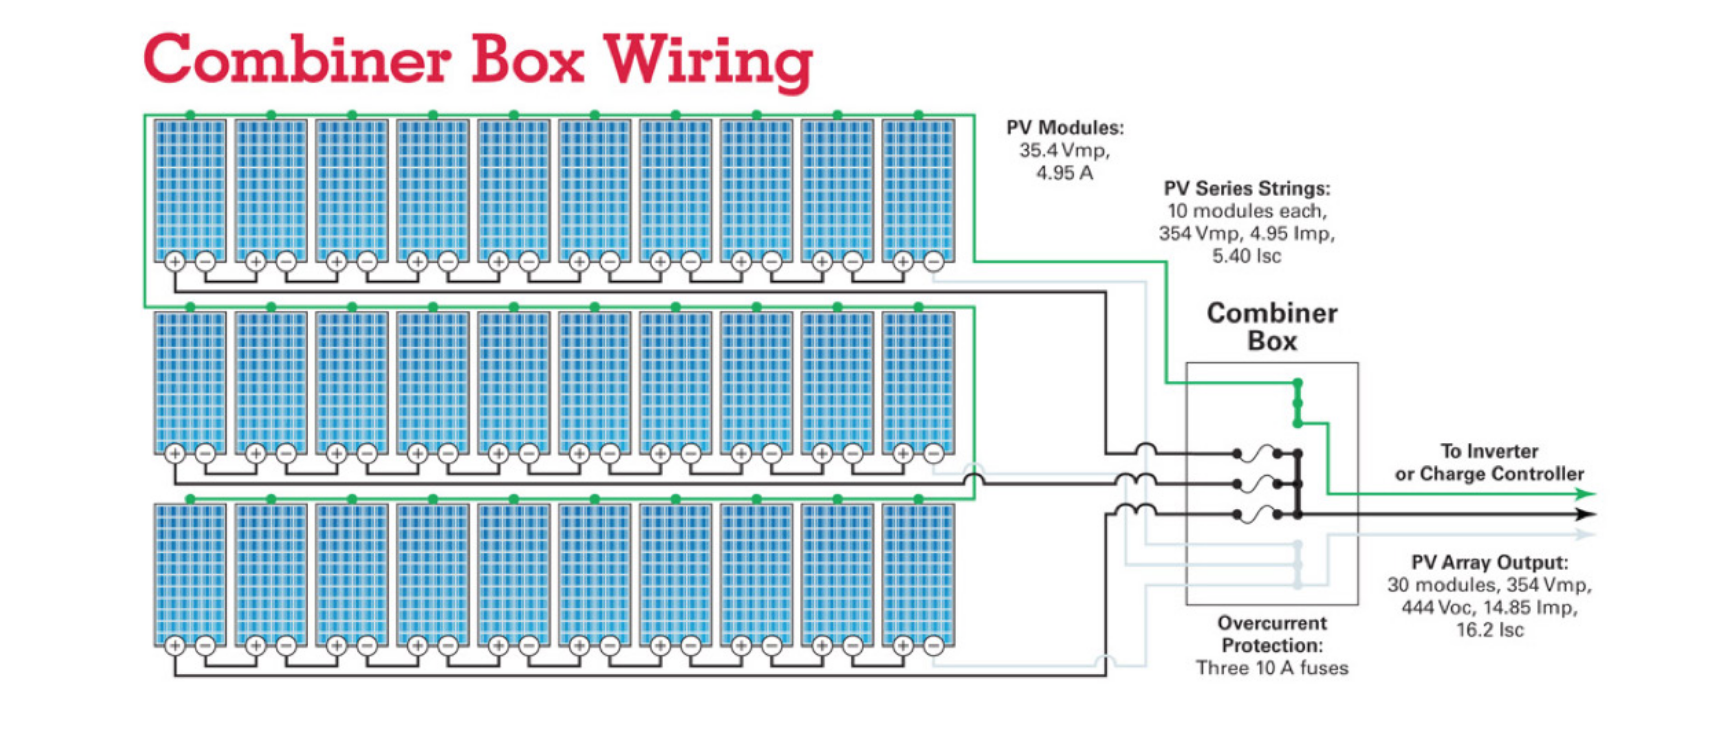
\includegraphics[width=\textwidth, keepaspectratio]{chapters/1_introduction/imgs/junctionbox.png}
    \caption{This figure represent an output circuit made of 3 string, each one hosts 10 solar modules.}
    \label{fig:outcircuit}
\end{figure}

%% @VP
%   qui c'è una parte che descrive i moduli di accumolo. Per
%   il modello non servono a nulla (che ci siano o no penso
%   sia indifferente). Lo aggiungo ?

\subsection{Inverter}
Energy from an array or a battery bank is direct current
(DC). This will provide for DC loads such a lights, fans,
pumps, motors, and some specialty equipment. However,
if the energy is to be used to power loads that operate on
alternating current (AC), as what is found in a residence, the
current needs to be converted. The inverter changes DC energy
to AC energy. Inverters are available in many different sizes
for various-sized loads. 
A string inverter is used to convert DC power from a solar
array to AC power and can be connected to an AC distribution
power panel (service panel) in a residence or facility.

%% @VP
%   qui c'è una parte sul PV Disconnect, uno strumento in grado
%   di disconnettere in sicurezza l'impianto. Ce lo metto ?

\subsection{System Metering}
Several tools are available to help the solar user to monitor
their system. On stand-alone or off-grid PV systems, the
battery meter is used to measure the energy coming in and
going out of the battery bank. Charging and discharging of
batteries, and proper functioning of the charging system is
important to alert the user to incomplete charging, battery
decline, or possible system shutdown. System monitoring
with web-based tools and apps allow the solar user to see
system activity using a cell phone or tablet from a location
away from their system.